\documentclass{article}

% Language setting
% Replace `english' with e.g. `spanish' to change the document language
\usepackage[czech]{babel}

% Set page size and margins
% Replace `letterpaper' with`a4paper' for UK/EU standard size
\usepackage[letterpaper,top=2cm,bottom=2cm,left=3cm,right=3cm,marginparwidth=1.75cm]{geometry}

% Useful packages
\usepackage{amsmath}
\usepackage{amsthm}
\usepackage{mathrsfs}
\usepackage{amsfonts}
\usepackage{amssymb}
\usepackage{graphicx}
\usepackage{caption}
\usepackage{mathbbol}
\usepackage[colorlinks=true, allcolors=blue]{hyperref}

% Uprava pro balicek mathbbol
\DeclareSymbolFontAlphabet{\mathbbm}{bbold}
\DeclareSymbolFontAlphabet{\mathbb}{AMSb}

\setlength\parindent{0pt}

\title{Modelování extrémních událostí}
\author{Vojtěch Obhlídal, Filip Mairinger}

\newtheorem{theorem}[subsubsection]{Věta}
\newtheorem{lemma}[subsubsection]{Lemma}

\theoremstyle{remark}
\newtheorem*{remark}{Poznámka}

\theoremstyle{plain}
\newtheorem{dusl}[subsubsection]{Důsledek}

\theoremstyle{definition}
\newtheorem{definition}[subsubsection]{Definice}

\theoremstyle{remark}
\newtheorem*{example}{Příklad}

\DeclareMathOperator{\sign}{sign}
\DeclareMathOperator*{\argmin}{arg\,min}
\DeclareMathOperator{\tg}{tg}


%stejnomerna konvregence
\def\cary{\buildrel\textstyle{\lower0.18pt\hbox{\smash-}}\over{\lower1.42pt\hbox{\smash-}}}
 
\def\rightarrowfill@x#1{\m@th\setboxz@h{$#1\cary$}\ht\z@\z@
  $#1\copy\z@\mkern-6mu\cleaders
  \hbox{$#1\mkern-2mu\box\z@\mkern-2mu$}\hfill
  \mkern-6mu\mathord\rightrightarrows$}
 
\newcommand{\xrightarrows}[2][]{
  \mathrel{\mathop{
    \setbox\z@\vbox{\m@th
      \hbox{$\scriptstyle\;{#1}\;\;$}
      \hbox{$\m@th\scriptstyle\;{#2}\;\;$}
    }
    \vbox{
    \kern-2pt
    \hbox to\wd\z@{\rightarrowfill@x\displaystyle}
    }
}
  \limits^{#2}\@ifnotempty{#1}{_{#1}}}
}
\newcommand{\nsk}[1]{\mathop{\not\xrightarrows{#1}}}


\begin{document}
\maketitle


\textbf{Státnicové otázky:}

\begin{enumerate}
    \item Detekce těžkých chvostů rozdělení, doba návratu události, čítací proces rekordů.
    \item Distribution-free nerovnosti a odhady hustot pro pravděpodobnostní chvosty.
    \item Semiparametrické a re-transformované odhady hustot, odhady vysokých kvantilů.
    \item Fluktuace náhodných sum, stabilní distribuce, zobecněný centrální limitní teorém, obor přitažlivosti, sub-exponenciální distribuce.
    \item Fluktuace náhodných maxim, Fisher-Tippettův zákon, oblasti přitažlivosti maxima, zobecněné Paretovo rozdělení.
\end{enumerate}


\section{Motivace}

Uvažujeme switch počítačové sítě s kapacitou $C$ a $n$ uživatelů tohoto switche. Abychom předešli přetížení sítě, využíváme řízení pomocí využití Call Admission Control (CAC), které zajišťuje přístup uživatelů do sítě tak, aby byla zajištěna určitá kvalita přenosu v síti, ale abychom připustili do sítě co největší množství uživatelů. Charakteristiky uživatelů jsou ale neznáme, popřípadě nemusí splňovat předem domluvené přenosové rychlosti. 
Uvažujme tedy množinu uživatelů $U = \{1,\dots,J\}$ a přenosové rychlosti $X_j(t)$ jakožto náhodné veličiny. Celkový přenos v daném čase je tedy dán veličinou agregovaného provozu $X(t) = \sum_{j=1}^{J} X_j(t)$. Maximální přenosovou kapacitu označíme $C$ a stupeň kvality systému $\gamma$. Cílem našeho zkoumání pak je, zda-li celkový přenos od všech uživatelů v síti překročí přenosovou kapacitu, tzn.
$$
\sum_{j=1}^{J} X_j(t) > C.
$$
Požadovaná kvalita systému by měla splňovat  podmínku
$$
\sup _{t} \mathbb{P}\left(\sum_{j=1}^{J} X_{j}(t)>C\right)<e^{-\gamma}.
$$
Naším cílem je pak odhadnout chvostovou pravděpodobnost, což je velmi málo pravděpodobná množina jevů (také řídké jevy). Abychom předešli překročení kapacity sítě, odhadujeme agregovaný provoz pomocí funkce parametrů uživatelů a tím řídíme přenos v síti.
$$
\mathbb{P}\left(\sum_{j=1}^{J} X_{j}>C\right)<F(\text { user parameters })<e^{-\gamma},
$$

Možné způsoby řízení jsou:

\begin{itemize}
    \item Peak Bit Rate Allocation - odhadneme pomocí součtu maximálních přenosových rychlostí uživatelů.
    \item Empirical bandwith - odhad pomocí experimentálně získaných výsledků.
    \item Rozdělením uživatelů do $M$ tříd podle přenosové kapacity následně lze omezovat počty uživatelů v jednotlivých třídách. Poté může provozovatel snižovat jednotlivým uživatelům rychlost za účelem udržení sítě v chodu, tzn. přesunout uživatele do jiné třídy. Toto lze snadno řešit pomocí strojového učení nebo neuronových sítí, jelikož klasifikujeme stavové vektory na povolené (uživatelé nepřesahují kapacitu) a nepovolené (uživatelé přesahují kapacitu).
\end{itemize}

Při řešení úlohy pomocí výše zmíněných metod se potýkáme s následujícími problémy:

\begin{enumerate}
    \item vysoká dimenze úlohy
    \item uživatelé nemusí dodržet přenosové deklarace, tzn. $X_i$ může nabývat vyšších hodnot než se předpokládalo
    \item \textbf{nedostatek dat ve chvostech}, což prakticky znemožňuje použití ML nebo NN pro predikci extrémních událostí
    \item vysoký výpočetní čas (v případě ML, NN)
    \item jedná se pouze o aproximaci
\end{enumerate}

Než přikročíme k distribution-free nerovnostem, představme dva typy chyb, které mohou nastat při přijímání uživatelů do sítě.

\begin{itemize}
    \item Tolerovatelná chyba - zamítnutí přístupu uživateli, který by síť nepřetížil
    \item Netolerovatelná chyba - přijetí uživatele, který síť přetížil a způsobil kolaps nebo zpomalení sítě
\end{itemize}

\newpage
\section{Distribution-free nerovnosti}

V této části nejprve uvedeme danou nerovnost, kterou následně aplikujeme na úlohu CAC.
Pro odhady pomocí distribution-free nerovností označme $m_j$ odhady středních hodnot přenosů jednotlivých uživatelů z minulého provozu. Dále označme $m_{2,j}$ jejich druhé momenty. Je třeba si uvědomit, že se jedná o takzvané online odhady, které se okamžitě přepočítávají. Jelikož je přenosová rychlost kladná, pak při aplikaci uvažujeme $X_j > 0 \; \forall j \in \hat{n}$ a tím pádem i  $\sum X_j > 0$. Navíc budeme uvažovat $\varepsilon = C$, aby mez odpovídala přenosové kapacitě sítě. Cílem pro nás bude určit parametr $\gamma$.

\subsection{Markovova nerovnost}
\begin{theorem}
Nechť $X$ je náhodná veličina, $X \in \mathscr{L}_1$. Pak pro $\forall \varepsilon > 0$ platí 
$$
\mathbb{P}\left( |X| \geq \varepsilon \right)  \leq \frac{\mathbb{E} |X|}{\varepsilon}.
$$
\end{theorem}


\textbf{Aplikace:}

$$
\mathbb{P}\left( \sum_{j=1}^{n} X_j > C \right) \leq \frac{1}{C}\mathbb{E} \left( \sum_{j=1}^{n} X_j \right) = \frac{1}{C}\sum_{j=1}^{n} \mathbb{E} X_j = \frac{1}{C}\sum_{j=1}^{n} m_j < \exp^{-\gamma}
$$

Tato nerovnost je ale nepřesná, což si můžeme uvést na příkladu náhodné veličiny $X \sim U(0,1)$ pro $\varepsilon = 1$. Pak odhadneme pravděpodobnost $\mathbb{P}\left(X \geq 1\right) \leq \frac{1}{2}$, což je ale velmi hrubý odhad, jelikož $\mathbb{P}\left(X \geq 1\right) = 0$.

\subsection{Čebyševova nerovnost}
\begin{theorem}
Nechť $X$ je náhodná veličina, $X \in \mathscr{L}_p$. Pak pro $\forall \varepsilon > 0$ platí 
$$
\mathbb{P}\left( |X| \geq \varepsilon \right)  \leq \frac{\mathbb{E} |X|^{p}}{\varepsilon^{p}}.
$$
\end{theorem}

\textbf{Aplikace: (pro $p = 2$)}

$$
\mathbb{P}\left( \sum_{j=1}^{n} X_j > C \right) \leq \frac{1}{C^{p}} \mathbb{E} \left( \sum_{j=1}^{n} X_j \right)^{2} = \frac{1}{C^{p}} \mathbb{E} \left( \sum_{j=1}^{n} X_j^{2} + \sum_{i \neq j} X_j X_i \right) \stackrel{p=2,\text{id}}{=} \frac{1}{C^{2}} \left( \sum_{j=1}^{n} m_{2,j} + \sum_{i \neq j}m_{j}m_{i}\right) < \exp^{-\gamma}
$$

Nutno zmínit, že tato nerovnost může být pro některé případy opět nepřesná a dává hrubé odhady.

\begin{remark}
Čebyševova nerovnost lze zapsat ve tvaru pro $X \in \mathscr{L}_2$. Tedy pro $\forall \varepsilon > 0$ platí 
$$
\mathbb{P}\left( |X - \mathbb{E}X| \geq \varepsilon \right)  \leq \frac{\mathbb{D}X}{\varepsilon^{2}}.
$$
Tato nerovnost ale posuzuje i odchylku od průměru agregovaného provozu "vlevo", která pro naši aplikaci není podstatná. Proto tato verze není vhodná pro naši úlohu, jelikož naším zájmem je pouze odchylka "vpravo".
\end{remark}

\subsection{Čebyševova-Cantelliho nerovnost}
\begin{theorem}
Nechť $X$ je náhodná veličina, $X \in \mathscr{L}_2$. Pak pro $\forall \varepsilon > 0$ platí 
$$
\mathbb{P}\left( X - \mathbb{E}X > \varepsilon \right)  \leq \frac{\mathbb{D} X}{\varepsilon^{2} + \mathbb{D} X} < \frac{\mathbb{D} X}{\varepsilon^{2}}.
$$
\end{theorem}

\begin{proof}
Předpokládáme BÚNO, že $\mathbb{E}X = 0$. Volíme $\varepsilon > 0$, dále 
$$
\varepsilon = \mathbb{E}\left(\varepsilon - X \right) \leq \mathbb{E}\left(\varepsilon - X \right)^{+} = \mathbb{E}\left(\left(\varepsilon - X \right) \mathbb{I}_{\{X \leq \varepsilon\}} \right)
$$

S využitím Cauchyho–Schwarzovy nerovnosti dostaneme
$$
\varepsilon^{2} = \left(\mathbb{E}\left[\left(\varepsilon - X \right) \mathbb{I}_{\{X \leq \varepsilon\}} \right]\right)^{2} \leq \mathbb{E}\left(\varepsilon - X \right)^{2} \cdot \mathbb{E}\left(\mathbb{I}_{\{X \leq \varepsilon\}}\right)^{2} = \left( \varepsilon^2 + \mathbb{E}X^2\right) \cdot \mathbb{P}\left(X \leq \varepsilon\right)
$$

Vyjádřením z této nerovnosti získáme 
$$
\mathbb{P}\left(X \leq \varepsilon\right) \geq \frac{\varepsilon^{2}}{\varepsilon^{2} + \mathbb{E}X^{2}}
$$
a dále
$$
\mathbb{P}\left(X > \varepsilon\right) \leq
1 - \mathbb{P}\left(X \leq \varepsilon\right) = \frac{\mathbb{E}X^{2}}{\varepsilon^{2} + \mathbb{E}X^{2}}.
$$
Nyní můžeme do nerovnosti dosadit libovolnou vycentrovanou náhodnou veličinu bez předpokladu na nulovost střední hodnoty, tedy
$$
\mathbb{P}\left(X = \mathbb{E}X > \varepsilon\right) \leq \frac{\mathbb{D}X}{\varepsilon^{2} + \mathbb{D}X}.
$$
\end{proof}

Získáme tak vylepšení Čebyševovy nerovnosti.

\textbf{Aplikace:}

$$
\mathbb{P}\left( \sum_{j=1}^{n} X_j > c \right) = \mathbb{P} \left( \sum_{j=1}^{n} X_j - \underbrace{\sum_{j=1}^{n} m_j}_{=m_A} > c - \underbrace{\sum_{j=1}^{n}m_j}_{=m_A}\right) \leq \frac{\mathbb{D}\left( \sum_{j=1}^{n} X_j\right)}{\mathbb{D}\left( \sum_{j=1}^{n} X_j\right) + \left(C - m_A\right)} < \exp^{-\gamma}
$$

Pokud předpokládáme nezávislost mezi jednotlivými uživateli, platí
$$
\mathbb{D}\left( \sum_{j=1}^{n} X_j\right) = \sum_{j=1}^{n}\mathbb{D} X_j = 
\sum_{j=1}^{n}\sigma_j^{2} =: \sigma_A^{2}, 
$$
kde $\sigma_A^{2}$ je agregovaný rozptyl.

Výhoda těchto nerovností je, že využívají jednoduché charakteristiky k odhadu. Navíc fungují i při nedostatku dat v chvostech (k extrémní události ještě nedošlo). Pro náhodné veličiny, které nemají definovanou střední hodnotu, popřípadě rozptyl (jako například Cauchyho rozdělení), nelze těchto nerovností využít.

\subsection{Chernoff bounding technique}
\begin{theorem}
Nechť $X$ je náhodná veličina a $h: \mathbb{R} \to \mathbb{R}^{+}$ je rostoucí funkce. Označme $Y = h(X)$. Pak pro $\forall \varepsilon > 0$ platí 
$$
\mathbb{P}\left(X \geq \varepsilon \right)  = \mathbb{P}\left(h(X) \geq h(\varepsilon) \right) \leq \frac{\mathbb{E} h(X)}{h(\varepsilon)}.
$$
Označíme-li $h(\varepsilon) = \varepsilon'$, získáme tím nerovnosti v kompaktnější verzi.
$$
\mathbb{P}\left(X \geq \varepsilon \right) \leq \frac{\mathbb{E} h(X)}{\varepsilon'}.
$$
\end{theorem}

\subsubsection{1. Chernoff bound}

Volme $s > 0$ libovolně, funkci $h(x) = e^{sx}$. Dosazením do Chernoffovy nerovnosti získáme

$$
\mathbb{P}\left(X \geq \varepsilon \right) \leq \frac{\mathbb{E}e^{sx}}{e^{s\varepsilon}}.
$$
Nyní můžeme optimalizovat výraz vpravo nalezením $s^{*} > 0$ tak, že

$$
\frac{\mathbb{E}e^{s^{*}x}}{e^{s^{*}\varepsilon}}
$$
je minimální. Dále si všimněme, že $m_X(s) = \mathbb{E}e^{sx}$ je momentová vytvářející funkce, jejíž existence nám dává první omezení na náhodnou veličinu $X$.

\textbf{Aplikace:}

$$
    \mathbb{P}\left( \sum_{j=1}^{n} X_j > c \right) = \frac{1}{e^{sC}} \mathbb{E} \left(e^{s\sum_{j=1}^{n} X_j}\right) \stackrel{\text{id}}{=} \frac{1}{e^{sC}} \prod_{j=1}^n \underbrace{\mathbb{E} e^{s X_j}}_{=m_{X_j}(s)}
    = e^{\sum_{j=1}^{n} \ln \mathbb{E} \left(e^{s X_j}\right) - sC} = e^{\sum_{j=1}^{n} \tilde{\mu}_j(s) - sC} < e^{-\gamma}
$$
Pomocí derivace podle parametru $s$ nalezneme minimum $s_{\text{opt}}^{*}$ a zpětně dosadíme do nerovnosti, čímž získáme horní hranice pro naši aplikaci na CAC. Pro výpočty odhadu může být nutné použít numerické metody.


\subsubsection{2. Chernoff bound}

Nechť $X > 0, s > 0$. Jako transformační funkci volíme $h(x) = xe^{sx}$.

\subsubsection{(n+1). Chernoff bound}

Nechť $X > 0, s > 0$. Jako transformační funkci volíme $h(x) = x^{n}e^{sx}$.

Odhad pravděpodobnosti má v tomto případě tvar

$$
\mathbb{P}\left( X \geq \varepsilon \right) \leq \frac{\mathbb{E}\left( X^{n} e^{sx} \right)}{\varepsilon^n e^{se}}
$$
pro libovolné $\varepsilon > 0$.

\begin{lemma}
Nechť $X$ je náhodná veličina, $\mathbb{E}X = 0$ a nechť $a \leq X \leq b$. Pak pro $\forall \varepsilon > 0$ platí 
$$
m_X(s) = \mathbb{E}\left(e^{sX}\right) \leq e^\frac{s^2 \left(b-a\right)^2}{8}.
$$
\end{lemma}

\begin{proof}[náznak]
Na intervalu $\left[a,b\right]$ je funkce $e^{sx}$ konvexní. Lze tedy rozepsat ve tvaru

$$
e^{sx} = \alpha e^{sb} + \left(1 - \alpha\right) e^{sa}
$$
pro $\forall x \in \left[a,b\right]$ a $\forall \alpha \in \left(0,1\right)$.

Pak volme $\alpha = \frac{x-a}{b-a}$ a

$$
\mathbb{E}\left(e^{sX}\right) = \frac{-a}{b-a} e^{sb} + \frac{b}{b-a}e^{sa} \leq e^{\frac{s^2 \left(b-a\right)^2}{8}},
$$
kde poslední nerovnost lze získat použitím metod matematické analýzy.
\end{proof}

Toto lemma můžeme použít v Chernoffově nerovnosti.

\textbf{Aplikace:}
Tuto aplikaci provedeme pro agregovanou veličinu $X_A$. Musíme uvažovat necentrovanou veličinu $X_A$, $\mathbb{E}X_A = m$.

$$
\mathbb{P}\left(X_A > C \right) = \mathbb{P}\left( X_A - m > C - m \right) \leq \frac{\mathbb{E} \left( e^s\left(X-m\right) \right)}{e^{\left(C-m\right)s}} \leq e^{\frac{s^2 \left(b-a\right)^2}{8} - \left(C-m\right)s}
$$

Následnou optimalizací získáme optimální hodnotu parametru

$$
s^{*} = \frac{4\left(C-m\right)}{\left(b-a\right)^2}.
$$
Výsledná nerovnost je pak ve tvaru

$$
\mathbb{P}\left(X_A > C \right) \leq e^{\frac{-2\left(C-m\right)^2}{\left(b-a\right)^2}} \leq e^{-\gamma}.
$$
Některé hodnoty mohou být neznáme a tak je třeba je nahradit vhodnými odhady, konkrétně pak střední hodnotu $\hat{m_A}$ a kraje intervalu $\hat{a}, \hat{b}$. Výraz $\left(b-a\right)^2$ pak nahrazuje rozptyl.

\subsection{H\"offdingova nerovnost}
Tuto nerovnost získáme nahrazením agregované veličiny sumou náhodných veličin v předchozí aplikaci, tedy

$$
X_A = \sum_{j=1}^n X_j.
$$

\begin{theorem}
Nechť $\left(X_j\right)_1^n$ jsou nezávislé náhodné veličiny z $\mathscr{L}_1$. Dále předpokládejme že platí $\left( X_j - \mathbb{E}X_j \right) \in \left[a_j,b_j\right]$ s.j. Potom pro $\forall \varepsilon > 0$ platí 

$$
\mathbb{P}\left(\sum_{j=1}^n X_j - m \geq \varepsilon \right) \leq e^{-\frac{2\varepsilon^2}{\sum \left(b_j-a_j\right)^2}},
$$
kde $m = \mathbb{E}\left(\sum_{j=1}^n X_j\right)$
\end{theorem}

\textbf{Aplikace:}

$$
\mathbb{P}\left(\sum_{j=1}^{n} X_j > C \right) = \mathbb{P}\left(\sum_{j=1}^{n} X_j - \underbrace{\sum_{j=1}^{n} m_j}_{=m} > C - m \right) \leq e^{\frac{-2\left(C-m\right)^2}{\sum_{j=1}^{n}\left(b_j-a_j\right)^2}} < e^{-\gamma}
$$

Opět je třeba odhadnout některé veličiny. Výsledné online řízení po sérii jednoduchých úprav dostaneme do tvaru

$$
\frac{2\left(C-\hat{m}\right)^2}{\sum_{j=1}^{n}\left(\hat{b_j}-\hat{a_j}\right)^2} > \gamma.
$$

Výhody a nevýhody H\"offdingovy nerovnosti:
\begin{itemize}
    \item Není potřeba znát rozptyly jednotlivých uživatelů, používáme omezení $\left[a_j,b_j\right] \; \forall j$. Na druhou stranu pokud je rozptyl výrazně menší než omezení $\left[a_j,b_j\right]$. pak jsou vhodnější nerovnosti používající rozptyl.
    \item Výpočetní čas k určení online řízení je v normě, není třeba používat numerické metody.
    \item Někdy může být nepřesná.

\end{itemize}

\begin{remark}[Bernsteinova nerovnost]
Nechť $\left(X_j\right)_1^n$ jsou nezávislé náhodné veličiny z $\mathscr{L}_2$. Dále předpokládejme že $\mathbb{E}X_j = 0$, $\mathbb{P}\left(X_j \leq l\right) = 1 \; \forall j \in \hat{n}$ a označme $\sigma_{AT}^2 = \sum_{1}^n \sigma_j^2$. Potom pro $\forall \varepsilon > 0$ platí 

$$
\mathbb{P}\left(\frac{1}{n}\sum_{j=1}^n X_j > \varepsilon \right) \leq e^{-\left(\frac{n\varepsilon^2}{2}\right)/\left(\frac{\sigma_{AT}^2}{n} + \frac{l\varepsilon}{3}\right)}.
$$
\end{remark}

\textbf{Aplikace:}

$$
\mathbb{P}\left(\sum_{j=1}^n X_j > C \right) = \mathbb{P}\left(\frac{\sum_{j=1}^n X_j - m_{AT} }{n} > \underbrace{\frac{C - m_{AT}}{n}}_{=K} \right) \leq e^{-\left(\frac{nK^2}{2}\right)/\left(\frac{\sigma_{AT}^2}{n} + \frac{lK}{3}\right)} < e^{-\gamma},
$$
kde $X_j - m_j \leq l \; \forall j$.

Výhody a nevýhody Bernsteinovy nerovnosti:
\begin{itemize}
    \item Hodnota $l$ je společná pro všechny přenosy ($\forall j$). To znamená, že kvůli jedinému uživateli může být potřeba extrémně široké pásmo.
    \item Jako u předchozích nerovností není třeba dat ve chvostech.

\end{itemize}
\newpage
\section{Odhady distribuce $X_{AT}$ (parameter-free)}
V této kapitole se zaměříme na tzv. \textit{parameter free} odhady, tedy na odhady distribuce pouze z naměřených dat

$$
\mathbb{P}\left(X_{AT} > C \right) = \underbrace{1 - F_{X_{AT}}\left(C \right)}_{\overline{F_X}\left(C\right)} \doteq 1 - \hat{F_{X}}\left(C \right) = \hat{\overline{F_X}}\left(C\right) < e^{-\gamma}, (CAC)
$$

kde neparametrický odhad $F_{X_{AT}}$ označíme $\hat{F_n}$.

\begin{remark}
 Platí $\mathbb{P}\left(X_{AT} > C \right) = R_X\left(C\right)$, což je spolehlivostní funkce v bodě $C$ (ze SKE).
\end{remark}

\subsection{Kvalita odhadu}
Při odhadu $\hat{F_n}$ chceme, aby fungoval pro libovolnou hodnotu $C$, tedy aby byl odhad stejnoměrně kvalitní. Požadujeme, aby platilo

$$
1 - \hat{F_n}\left(C \right) \xrightarrow{\mathbb{P}, s.j.} 1 - F\left(C \right) \quad \forall C > C_0 >\geq 0, \; C \leq C_F,
$$
kde hodnoty $C_0$, resp. $C_F$ jsou minimální, respektive maximální možná kapacita.

Požadujeme tedy, aby

$$
\sup_{C \geq 0} |\hat{F_n}\left(C \right) - F\left(C \right)| \xrightarrow{s.j.} 0 \quad \textnormal{(stejnoměrně)}.
$$

Povšimněme si, že toto supremum je Kolmogorovova vzdálenost, označíme tedy

$$
K\left( \hat{F_n},F \right) = \sup_{C \geq 0} |\hat{F_n}\left(C \right) - F\left(C \right)|.
$$
Jinými slovy tedy požadujeme, aby $\hat{F_n}$ byl konzistentní odhad (s.j.) v kolmogorovovské vzdálenosti $K$.

\smallskip

Zaměřme se nyní na kvalitu odhadu hustoty pravděpodobnosti $\hat{f_n}$. Tu totiž můžeme použít k odhadu chvostové pravděpodobnosti $\mathbb{P}\left(X > C\right)\int_{C}^{+\inf} \hat{f_n}(t) \,dt$.

Pro hustotu požadujeme, aby

$$K\left( \hat{F_n},F \right) \leq \frac{1}{2}V\left(\hat{f_n},f\right),
$$
kde $V\left(\hat{f_n},f\right)$ je $L_1$ norma a nazýváme ji \textbf{totální variace} (TV). Dále platí, že $V\left(\hat{f_n},f\right) \xrightarrow{s.j.} 0$. Hledáme tedy $\hat{f_n}$ tak, aby byla konzistentní v TV.

\subsection{Metody odhadu}
Ukažme si nyní různé možnosti odhadu jak distribuční funkce, tak i hustoty pravděpodobnosti.

\subsubsection{EDF}
Nechť $\left(X_j\right)_1^n \sim F$ jsou id (iid) náhodné veličiny.

\begin{definition}
Funkci
$$
F_n\left(t,\mathbb{X}\right) = \frac{1}{n} \#\{j:X_j \leq t\} = \frac{1}{n} \sum_{j=1}^{n} \text{I}_{(-\infty,t]}\left(X_j\right), \ \forall t \in \mathbb{R}
$$
nazveme \textbf{empirickou distribuční funkcí} (EDF).
\end{definition}

\begin{theorem}
Pro $F_n\left(t\right)$ platí, že je nestranným, konzistentním a asymptoticky normálním odhadem funkce $F\left(t\right)$. Navíc $F_n \overset{\mathbb{R}}{\rightrightarrows}F \ \text{s.j.}$
\end{theorem}

\begin{figure}[h]
    \centering
    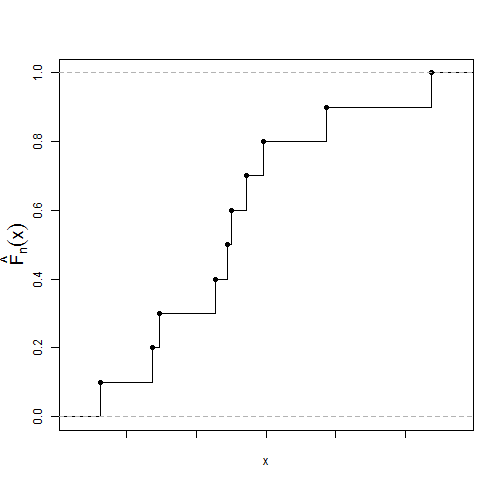
\includegraphics[scale=0.8]{pics/EDF.png}
    \captionsetup{justification=centering}
    \caption{Emprická dsitribuční funkce $\hat{F_n}$. \\ 
    a) Pokud nemáme data ve chvostu, odhadujeme $F_{X_{AT}}(C) \doteq 1 - \hat{F_n}(C) = 0 < e^{-\gamma}$ pro $C \in [x_{(n),1}]$ \\
    b) Derivací EDF nelze získat odhad PDF, jelikož $\hat{f_n} = \frac{d}{dt}F_n = 0$ s.v.}
\end{figure}


\subsubsection{Odhad hustot}

\begin{definition}
Nechť $\exists f$ pro $X \sim F$. Definujeme \textbf{empirickou hustotu pravděpodobnosti} (EPDF) vztahem
$$
f_n\left(t,\mathbb{X}\right) = \frac{F_n\left(t + \lambda_n\right) = f_n\left(t - \lambda_n\right)}{2\lambda_n}, \ \forall t \in \mathbb{R}, \ \text{kde} \ \left(\lambda_n\right)_1^{\infty} > 0.
$$
\end{definition}

Empirická hustota pravděpodobnosti splňuje řadu vlastností, které shrneme v následující větě.

\begin{theorem}
Pro $f_n(t)$ platí, že je asymptoticky nestranným a konzistentním odhadem funkce $f(t)$, pokud je splněno $\lambda_n \rightarrow 0$ a $n\lambda_n \rightarrow +\infty$. Pokud navíc $n\lambda_n^3 \rightarrow 0$, je $f_n(t)$ také asymptoticky normálním odhadem $f(t)$.
\end{theorem}

\subsection{Přehled neparametrických metod odhadů hustot pravděpodobnosti (PDF)}

\subsubsection{Fixed Partition Histogram (FPH)}

Předpokládáme, že $X \sim f$, kde $f$ je skutečná hustota veličiny $X$ a $\text{supp}(f) \subset [a,b]$. Dále si zavedeme dělení intervalu $[a,b]$ na $B_j = [a_j,a_{j+1}), \ \forall j \in \hat{m}$, ozn. $h=\lambda(B_j) \ \forall j$. Lze navíc uvažovat ne-ekvidistantní dělení a brát různé velikosti binů. Dále označme
$$
Y_j = \#\{i:X_i \in B_j\} = \sum_{i=1}^n \text{I}_{\{X_i \in B_j\}}, \ \forall j.
$$

\begin{definition}
Nechť pro $\forall t \in B_j$ platí

$$
\hat{f_n^H}(t) = \frac{1}{nh} \sum_{i=1}^n \text{I}_{\{X_i \in B_j\}} = \frac{1}{nh} \sum_{j=1}^m Y_j \mathbb{1}_{\{t \in B_j\}}, \ \forall t \in [a,b]
$$
pro ekvidistantní dělení intervalu. Pro ne-ekvidistantní dělení musím vzorec pozměnit do tvaru

$$
\hat{f_n^H}(t) = \frac{1}{n} \sum_{i=1}^n \frac{1}{h_j} \text{I}_{\{X_i \in B_j\}},
$$
kde $h_j = \lambda(B_j)$.

\end{definition}

\begin{theorem}[Vlastnosti odhadu]
Pro histogramový odhad platí následující
\begin{enumerate}
    \item odhad $\hat{f_n^H}$ je Lebesgueovskou hustotou
    \item odhad $\hat{f_n^H}(t)$ je asymptoticky nestranný odhad $f(t), \ \forall t \in \mathbb{R}$ pro $h_n \rightarrow 0$
    \item $\operatorname{Var} \hat{f_n^H}(t) \rightarrow 0$ pro $\forall t$, pokud $h_n \rightarrow 0$ a $nh_n \rightarrow +\infty$
    \item $\hat{f_n^H}$ je konzistentní odhad pro $f(t)$, $\forall t$
    \item $\hat{f_n^H}$ je AN odhad $f(t)$, $\forall t$, pokud $h_n \rightarrow 0$, $nh_n \rightarrow +\infty$, $nh_n^3 \rightarrow 0$ a $f$ diferencovatelná v $t$
    \item lze ukázat, že pro IMSE (Integrated Mean Squared Error), definovanou vztahem \\ $\operatorname{IMSE}(\hat{f_n^H},f) = \int_{\mathbb{R}} \mathbb{E}_f(\hat{f_n^H}(t)-f(t))^2 dt = \mathbb{E}_f \int_{\mathbb{R}} (\hat{f_n^H}(t)-f(t))^2 dt$, platí $\operatorname{IMSE} \rightarrow 0$ pro $h_N \rightarrow 0$ a $nh_n \rightarrow +\infty$
\end{enumerate}
\end{theorem}

Pro IMSE je navíc znám i řád konvergence, který je $\operatorname{IMSE} = \mathcal{O}(n^{-2/3})$ při $h_n \rightarrow 0$, $nh_n \rightarrow +\infty$ a $nh_n^3 \rightarrow 0$ a pro $f$ diferencovatelnou. Optimální šířka ekvidistantního binu je pak

$$
h_n^{*(IMSE)} = h_n^* = \left(
\frac{6}{\int (f')^2}\right)^{1/3} \cdot n^{-1/3}.
$$

Pokud navíc $f \sim \text{N}(\mu,\sigma^2)$, pak $h_n^* = 3.49\sigma \cdot n^{-1/3}$, kde ale hodnotu $\sigma$ neznáme. Proto odhadujeme pomocí výběrového rozptylu $s_n$, tedy $\hat{h_n^*} = 3.49 s_n \cdot n^{-1/3}$. Připomínáme, že $s_n^2 = \frac{1}{n-1} \sum_{i=1}^n (X_j - \overline{X_n})^2$. Jelikož není tento odhad robustní na data velmi odchýlena od průměru, proto lze použít robustnější variantu (Diaconis,1981), která je $h_n^* = 2(\text{IQR} \cdot n^{-1/3})$, kde IQR je inter-kvartilové rozpětí. \newline

Pro CAC, Devroye a Gy\"orfi (1985) ukázali $\text{L}_1$-konzistenci (v totální variaci) a navíc pro MIAE (nebo IMAE, mean integrate absolute error) platí

$$
\text{IMAE} = \int \mathbb{E}_f |\hat{f_n^H - f}| dt = \mathcal{O}(n^{-1/3}).
$$

Oproti IMSE se jedná o poměrně pomalou konzistenci. Nevýhody této metody:

\begin{itemize}
    \item nespojitost odhadované hustoty
    \item omezený support odhadované hustoty, takže chybí chvosty (zejména při nedostatku dat)
    \item závislost na dělení a velikosti binů $h_n$
\end{itemize}

\subsubsection{Jádrový odhad hustoty (Kernel density estimation)}

Nechť $X \sim f, h_n > 0$. Pak definujeme jádrový odhad hustoty
$$
\hat{f_n}^K(t) = \frac{1}{nh_n} \sum_{i=1}^n K\left(\frac{t-X_i}{h_n}\right),
$$
kde $K$ nazýváme jádro a platí pro něj $K(u) \geq 0$ a $\int K(u) du = 1$. Hodnotu $h_n > 0$ nazýváme vyhlazovacím parametrem (smoothing parameter) nebo šířkou okna (window width). Platí, že $\hat{f_n}^K$ je Lebesgueovská hustota. \newline

Jako jádro můžeme volit následující hustoty:

\begin{enumerate}
    \item jádro typu $K(u) = \kappa_{r,s} (1-|u|^r)^s \text{I}_{[-1,1]}(u)$
    \begin{itemize}
        \item obdélníkové $(s=0,\kappa_{r,s}=1/2)$: $K(u) = \frac{1}{2} \text{I}_{[-1,1]}(u)$
        \item trojúhelníkové $(s=0,r=1,\kappa_{r,s}=1)$: $K(u) = \left(1-|u|\right)^s\text{I}_{[-1,1]}(u)$
        \item Bartlett-Epanechnikov $(s=1,r=2,\kappa_{r,s}=3/4)$: $K(u) = \frac{3}{4} \left(1-|u|^2\right)\text{I}_{[-1,1]}(u)$
        \item biweight $(s=2,r=2,\kappa_{r,s}=15/16)$
        \item triweight $(s=3,r=2,\kappa_{r,s}=35/32)$
    \end{itemize}
    \item Gauss $K(u) = \frac{1}{\sqrt{2\pi}} e^{-u^2/2}, u \in \mathbb{R}$, které má neomezený nosič (a proto $\hat{f_n}^K$ má potom nenulové chvosty při aplikaci na CAC)
    \item Laplace $K(u) = \frac{1}{2} e^{-|u|}, u \in \mathbb{R}$, opět s neomezeným nosičem
\end{enumerate}


Doporučená volba pro $\hat{h_n^{*IMSE}}$ je

\begin{equation}
    {h_n^*}^{\text{IMSE}} = \left[ \frac{\int K(u)^2 du}{(\int u^2 K(u)du)^2} \frac{1}{\int f''(u)^2 du} \right]^{1/5} n^{-1/5},
\end{equation}

\smallskip

kde $K \in \mathcal{L}_2$, $0 < \mathbb{E}^k(u^2) < + \infty$ a $f \in C^{(2)}$. \newline Pro $X_{AT} = \sum_{j=1}^n X_j \sim F$, kde $f$ je skutečná hustota, vede na řád

$$
\text{IMSE} = \mathcal{O}(n^{-4/5}),
$$

což vylepšuje histogram. Pro volbu $K \sim \text{N}(0,1), f \sim \text{N}(\mu,\sigma ^2)$ dostáváme hodnotu $h_n^* = 1.06 \cdot \sigma \cdot n^{-1/5}$, kterou odhadujeme $\hat{h_n^*} = 1.06 \cdot s_n \cdot n^{-1/5}$.

Pro long-tailed distribuce (sešikmené distribuce, těžší chvosty) je doporučeno (Silverman, 1986)
$$
h_n^* = 0.79 \cdot (\hat{\text{IQR}}) \cdot n^{-1/5},
$$
kde $\hat{\text{IQR}}$ je odhad interkvartilové rozpětí.

Lze také volit kompromis 
$$
h_n^* = \min \left(s_n ,\frac{\hat{\text{IQR}}}{1.34}\right) \cdot 0.9 \cdot n^{-1/5},
$$
ale jsou i další možnosti voleb. Optimálním jádrem $K$ z hlediska asymptotické IMSE je jádro Epanechnikovo (1969). Dále $L_1$-konzistence (Devroye, 1983)

$$
\operatorname{IMAE} = \mathcal{O}(n^{-2/5})
$$

dosahuje lepších výsledků než histogram.

\bigskip

Uvažujeme $X \sim f$ hustotu v $\mathbb{R}^d$, $K(u)$ je symetrická hustota a $f''$ je spojitá a omezená. Pak definujeme 

$$
\hat{f_n^k}(t) = \frac{1}{n h_n^d} \sum_{j=1}^n K\left(\frac{t-X_j}{h_n}\right), \quad \forall t \in \mathbb{R}^d.
$$

Doporučená volba je pak $h_n^* = \mathcal{O}(n^{-\frac{1}{d+4}})$ a dosahujeme řádu 

$$
\text{IMSE} = \mathcal{O}(n^{-\frac{1}{d+4}}),
$$
t.j. například pro $d=1: \ \text{IMSE} \sim \frac{1}{\sqrt[5]{n^4}}$, $d=36: \ \text{IMSE} \sim \frac{1}{\sqrt[10]{n}}$. Narážíme na \textit{prokletí dimensionality} a pro vyšší dimenze je třeba obrovské množství dat. V následující tabulce je porovnání potřebného množství dat pro různé dimenze, abychom dostali srovnatelné odhady.

\begin{table}[h]
\centering
    \begin{tabular}{|c|ccccc|}
    \hline
    Dim $d$ & 1 & 3 & 5 & 7 & 10 \\   \hline
    $n$ & 4 & 67 & 768 & 10700 & 842000 \\ \hline
    \end{tabular}
    \caption{Potřebný počet dat pro danou dimenzi, aby byly odhady srovnatelné.}
    \label{table:dim_n}
\end{table}

Návrhy pro jádra v $d$-rozměrných prostorech.

\begin{itemize}
    \item Gaussovo jádro
    $$
    K(\mathbbm{u}) = \frac{1}{(\sqrt{2\pi})^d} e^{-\frac{1}{2}\mathbbm{u}^T\mathbbm{u}}
    $$
    \item Bartlett-Epanechnikovo jádro
    $$
    K(\mathbbm{u}) = \kappa (1-{\mathbbm{u}^T\mathbbm{u})}^p \text{I}({\mathbbm{u}^T\mathbbm{u} \leq 1}) \; \text{, kde } \; p = 2,3
    $$
\end{itemize}

Po výběru jádra musíme řešit bias-variance trade-off.

\begin{equation*}
\begin{aligned}
 \text{MSE}(\hat{f_n^k}) &= \mathbb{E}(\hat{f_n^k}(t) - f(t))^2 = \lVert \hat{f_n^k} - f\rVert = \lVert \hat{f_n^k} - \mathbb{E}\hat{f_n^k} + \mathbb{E}\hat{f_n^k} - f\rVert_{L_2} \leq \lVert \hat{f_n^k} - \mathbb{E}\hat{f_n^k}\rVert_{L_2} + \lVert \mathbb{E}\hat{f_n^k} - f\rVert_{L_2}  \\ &= \mathbb{E}(\hat{f_n^k} - \mathbb{E}\hat{f_n^k})^2 + \mathbb{E}(\mathbb{E}\hat{f_n^k} - f)^2 = \text{Var}(\hat{f_n^k}) + \left[\text{Bias}(\hat{f_n^k})\right]^2  
\end{aligned}
\end{equation*}

Dále je třeba najít vhodný poměr (trade-off) mezi oběma členy z předchozího výrazu, které mají protichůdné vlivy proti vyhlazovacímu parametru. (OBRAZEK)

\subsection{Vylepšení odhadů}

Dále diskutujme možnosti vylepšení histogramu a jádrového odhadu.

\subsubsection{Variable Partition Histogram}

Hledáme odhad $f_n^{VPH}$, pro který je třeba zavést dělení na biny v závislosti na $n$ a samotných datech.

Vytváříme binování, které tvoří support $\{A_{n,i}\}:$ 
$$
A_{n,1} = \left[X_{(1)},X_{(k)}\right],
A_{n,2} = \left(X_{(k)},X_{(2k)}\right],
\dots,
A_{n,2} = \left(X_{((l-1)k)},X_{(lk)}\right],
$$
kde $n = lk$. Volíme různé délky binů tak, abychom zamezily problému s nedostatkem dat.
$$
h_{n,i} = \lambda(A_{n,i}); \hat{f}_n^{VPH}(t) = \frac{k}{n} \frac{1}{h_{n,i}} \forall t \in A_{n,i}
$$

\subsubsection{k-NN odhad $f$ (Nearest neighbour)}

Odhadujeme hustotu

$$
\hat{f_n}^{NN}(t) = \frac{k}{n} \frac{1}{\mu(B_d(t,d_k(t)))},$$
kde
$B_d(t,d_k(t))$ je $d$-dimenzionální koule se středem v $t$ a poloměrem $d_k(t)$, což je vzdálenost $t$ ke $k$-tému nejbližšímu sousedovi v datech $X_j$. Tento odhad prodlužuje chvosty i za data, což je výhodné pro CAC.

\subsubsection{Adaptivní kernel}

Definujeme odhad s adaptivním jádrem vztahem

$$
\hat{f_n^{AK}}(t) = \frac{1}{n} \sum_{i=1}^n \frac{1}{h_i^{d}} K\left(\frac{t-x}{h_i}\right), \forall t \in \mathbb{R}^d,
$$
kde značíme $h_i = h_{n,i}$.

Volba $h_i$ je dvou-krokový odhad: $\widehat{f_n} \rightarrow h_i(\widehat{f_n}(x_i)) \rightarrow \widehat{f_n^{AK}}$, kde $\hat{f_n}$ je pilotní odhad, na jehož základě získáme pomocí $h_i$ binování pro adaptivní kernel. Podle Silvermana (1986) je postup následující:

\begin{enumerate}
    \item volíme pilotní $h_p$, $K$ libovolné (například Gaussovo, Epanechnikovo) a vytvoříme pilotní odhad $\widehat{f_n^K}$
    \item (mezikrok) $h_i = h_p\left(\frac{1}{g}\widehat{f_n^K}(X_i)\right)^{-\alpha}$, kde $\alpha \in (0,1)$ je sensitivity parameter, podle Silvermana: $\alpha=1/2$, $g$ je geometrický průměr z hodnot $\left(\widehat{f_n^K(X_i)}\right)_1^n$
    \item pomocí $h_i$ napočítáme $\widehat{f_n^{AK}}$
\end{enumerate}

\newpage

\begin{remark}
Komentář k AKDE (\textit{Adaptive kernel density estimation}):
\begin{enumerate}
    \item $\widehat{f}_{n,\textnormal{pilot}}^K$ $\Rightarrow$ volba $h_i$ $\Rightarrow \widehat{f}_n^{AK}$ (není třeba zachovávat stejné jádro!)
    \item Lehké zobecnění od Hall $\&$ Marron (1988):\ \newline Při ladění $h_i$ používají $h_i=h\big(\widehat{f}_{n,h_{\textnormal{pilot}}}^K(x_i)\big)^{-\frac{1}{2}(=\alpha)}$, kde $h_{\textnormal{pilot}}$ je vyhlazovací parametr pilotního odhadu a $h$ je volitelný parametr do AKDE
    \item Jak tedy vypadá jádrový odhad, když se takto zvolí $h_{\textnormal{pilot}}$ a $h$?
    \begin{equation}
        \widehat{f}_n^{AK}(t|h_{\textnormal{pilot}},h)=\frac{1}{nh}\sum_{i=1}^n \big(\widehat{f}^K_{n,h_{\textnormal{pilot}}}(x_i)\big)^{\frac{1}{2}}\cdot K\left(\frac{t-X_i}{h}\cdot\left(\widehat{f}^K_{n,h_{\textnormal{pilot}}}(x_i)\right)^{\frac{1}{2}}\right)
        \label{HallMarron}
    \end{equation}
\end{enumerate}
\end{remark}

\begin{theorem}[Vlastnosti \eqref{HallMarron}]
Nechť $f\in C^{(4)}$ a $f$ je lokané odražená od 0. Nechť dále platí, že \newline$\int K^2 < +\infty$ a jádro $K$ je omezené atd. Potom pokud volíme $h_{\textnormal{pilot}}=c_1n^{-\frac{1}{5}}$, $h=c_2n^{-\frac{1}{9}}$, pak\newline (I)MSE$(\widehat{f}^{AK}_n)=\mathcal{O}(n^{-\frac{8}{9}})$.
\end{theorem}

\section{Re-transformované neparametrické odhady hustot}

\subsection{Algoritmus}
\begin{enumerate}
    \item Máme $X\sim f_X$ a získáme data $\textbf{X}$ iid $f/F$
    \item Volíme vhodnou transformaci $T:\mathcal{X}(\mathbb{R})\to\mathcal{Y}(\mathbb{R})$ a předpokládejme, že $T$ je ryze monotónní (dále BÚNO ostře rostoucí)
    \item Transformujeme data: $Y_j=T(X_j)$ pro všechna $j\in\widehat{n}$, kde $Y_j$ iid $g/G$\newline
    $G(y)=P(Y_1\leq y)=P(X_1\leq T^{-1}(y))=F(T^{-1}(y))$
    \item Hustota, kterou chceme po této transformaci odhadovat je $g(y)=f(T^{-1}(y))\cdot\left(T^{-1}(y)\right)'$ (volíme transformaci tak, aby $g$ byla vhodnější než $f$), cíl tedy je, aby $g$ byla omezená a aby i přípustný nosič $g$ byl omezený
    \item $\widehat{g}_n(y)$ neparametrický odhad $g$ (lze i parametricky) z dat $(Y_j)_{j=1}^n$ iid $g$
    \item normalizace $\widehat{g}_n(y)$ na $\textnormal{supp}(g)=\mathcal{Y}$
    \item $T^{-1}$ zpět na $\widehat{f}_n^{RT}(x)=\widehat{g}_n(T(x))\cdot T'(x)$
\end{enumerate}
\vspace{0.2cm}

\subsection{Praxe} Neznáme $f$, tedy nevíme, jako volit transformaci $T$.
\vspace{0.35cm}

\subsection{Kvalita} 
\begin{align*}
    \textnormal{IMSE}(\widehat{f}_n^{RT})&=E\int_\mathcal{X}\left(\widehat{f}_n^{RT}(x)-f(x)\right)^2dx=E\int_\mathcal{X}\big[(\widehat{g}_n(T(x))-g(T(x))\big]^2\cdot \left(T'(x)\right)^2dx= \\
    &=\bigg|\begin{array}{c}
         y=T(x)\\
         dy=T'(x)\,dx 
    \end{array}\bigg|=E\int_\mathcal{Y}\big[\widehat{g}_n(y)-g(y)\big]^2\cdot T'\big(T^{-1}(y)\big)\,dy= \\
    &=\int_\mathcal{Y}\underbrace{T'\big(T^{-1}(y)\big)}_{0<\dots<c\footnotemark{}}\cdot \underbrace{E\big(\widehat{g}_n-g\big)^2}_{\textnormal{MSE}(\widehat{g}_n)}dy\leq c\cdot \textnormal{IMSE}(\widehat{g}_n) \\
    &\Rightarrow \textnormal{ Řád IMSE}(\widehat{f}_n^{RT}) \textnormal{ je stejný jako IMSE}(\widehat{g}_n)!
\end{align*}
\footnotetext{Transformaci $T$ volíme tak, aby byla omezená.}

\begin{align*}
    \textnormal{MIAE}(\widehat{f}_n^{RT})\textnormal{ shodný s MIAE}(\widehat{g}_n)\,\,\,\,\textnormal{(DCv - }L_1\textnormal{ norma je invariantní na transformace dat/hustot)}
\end{align*}

\subsection{Volba transformace dle Devroye \& Györfi (1985)}

Pro veličinu $X\geq 0$ navrhují transformaci $T:\mathbb{R}^+\to\langle 0,1\rangle$ následovně:
\begin{align*}
    y=T(x)=\begin{cases}
    \sqrt{\frac{F(x)}{2}} & \textnormal{pro }F(x)\leq 0,5 \\
    1-\sqrt{\frac{1-F(x)}{2}} & \textnormal{jinak.} \\
    \end{cases}
\end{align*}

\begin{figure}[h]
    \centering
    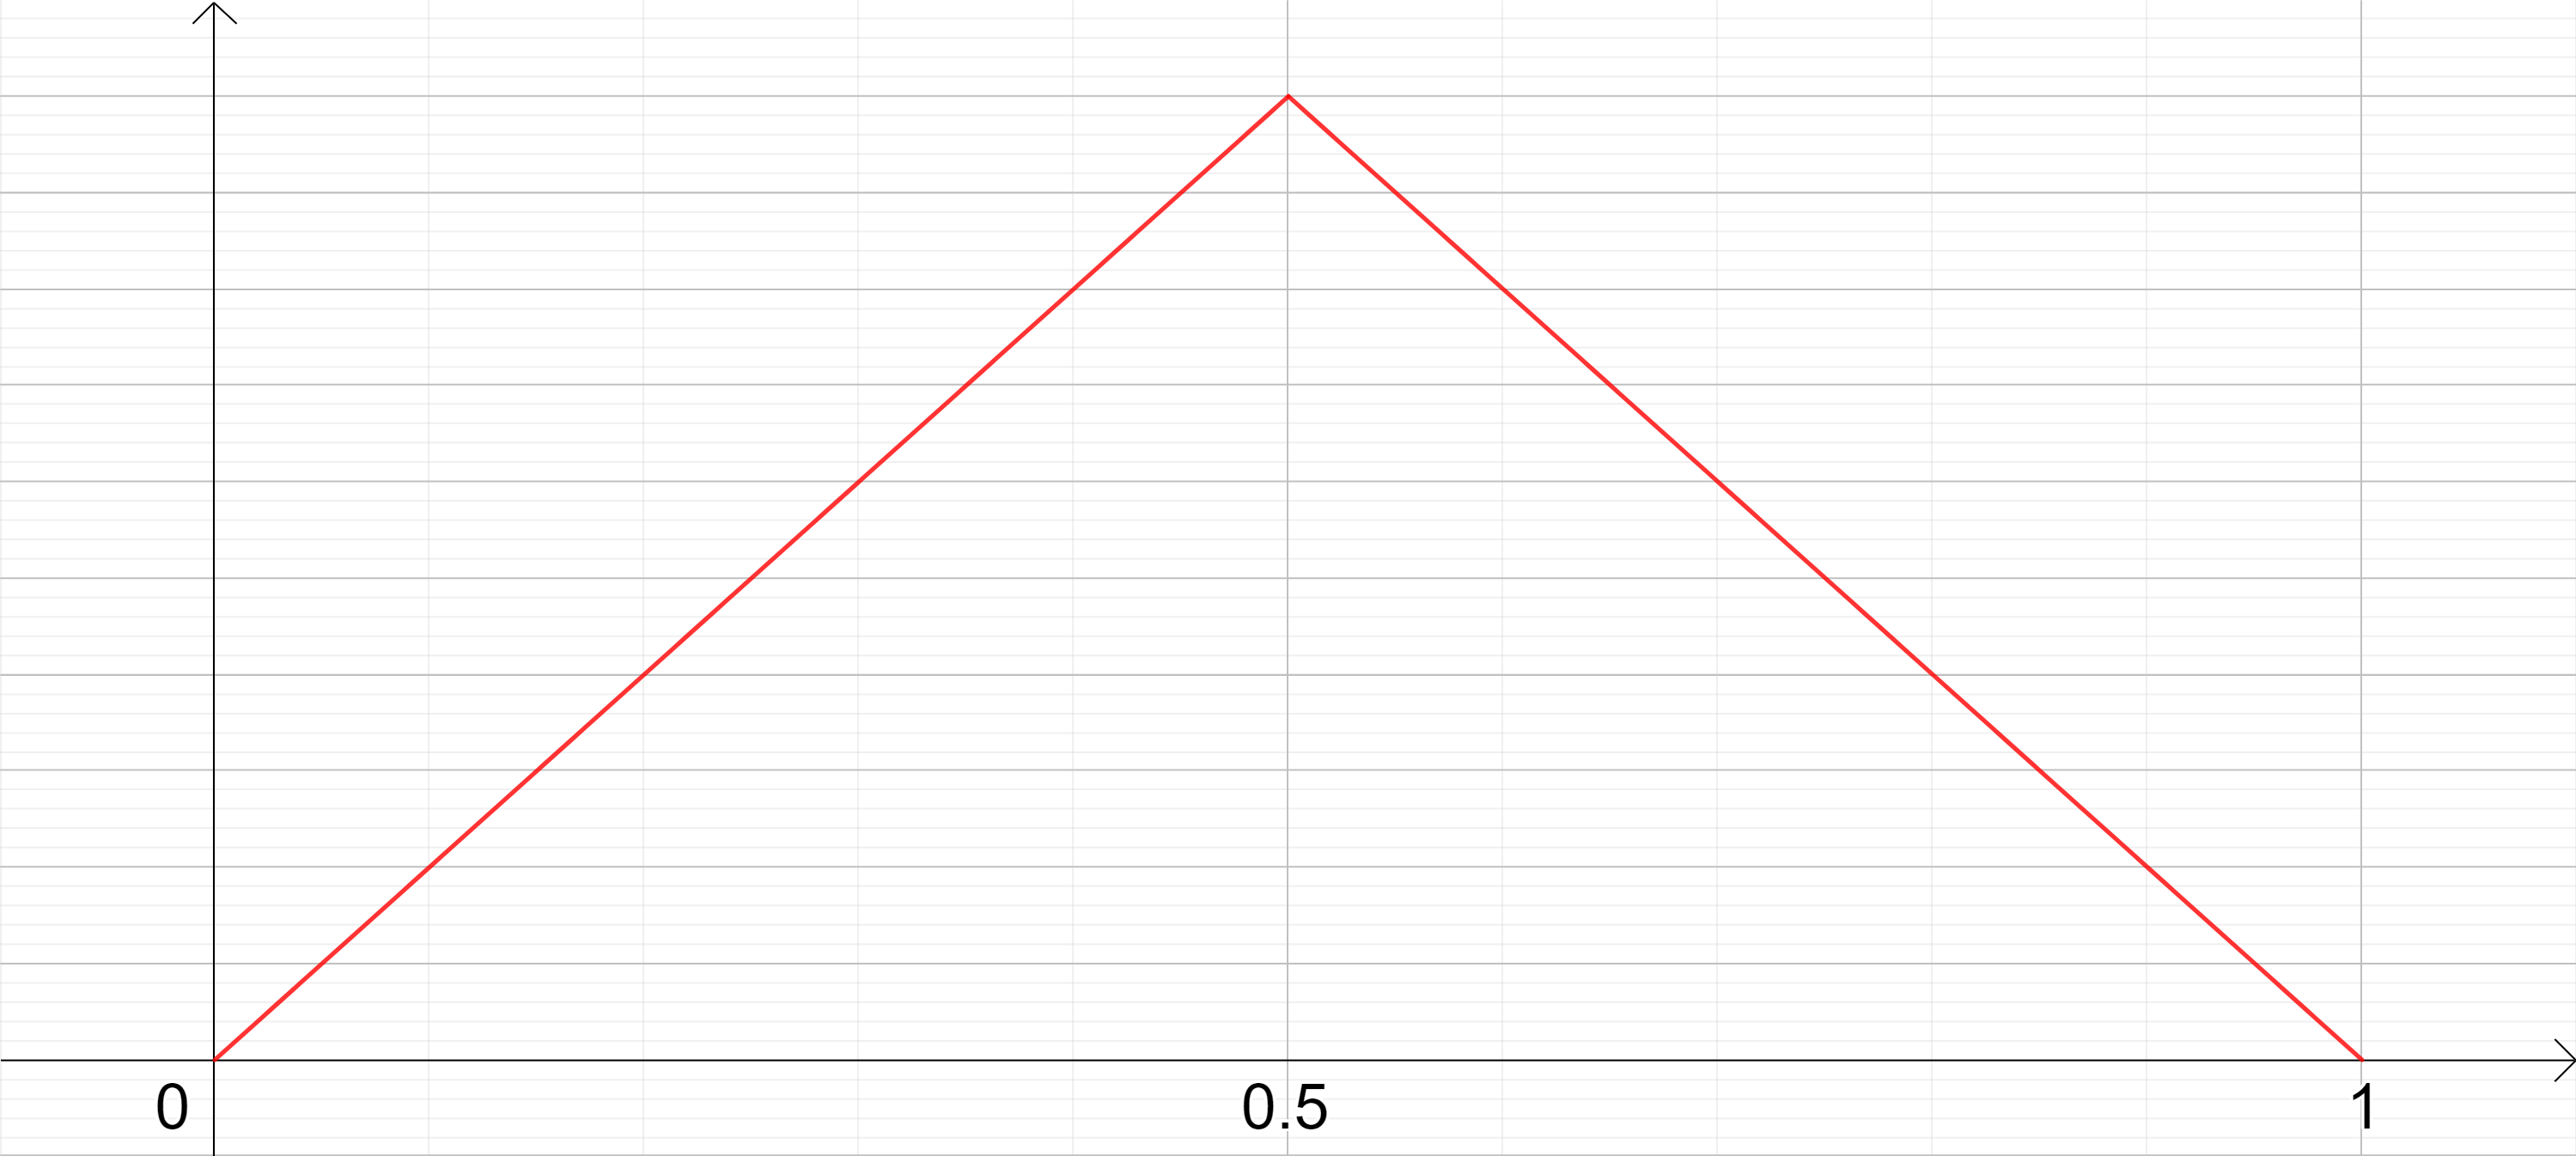
\includegraphics[scale=9]{pics/rovnoramenna_hustota.png}
    \caption{Transformovaná hustota $g$ ($f\xrightarrow{T}g$)}
\end{figure}

\subsection{Volba transformace dle Yang \& Marron (1999)}

\begin{align*}
    T_\lambda(x)=\begin{cases}
    x^\lambda\sign(\lambda) & \textnormal{pro }\lambda\neq 0 \\
    \ln x & \textnormal{pro }\lambda=0 \\
    \end{cases}
\end{align*}

Parametr $\lambda$ se ladí tak, aby $\lambda=\argmin_{\lambda} \int \left(g_\lambda''(y)\right)^2dy$.

\subsection{Volba transformace dle Markovitch \& Krieger (2000)}

\begin{align*}
    T(x)=\frac{2}{\pi}\arctan x
\end{align*}

Problém s omezeností $g(y)$ po transformaci (například pro Weib$(\lambda,\alpha<1)$).

\section{Semiparametrické odhady hustot}

\begin{enumerate}
    \item Kombinované 1: $\widehat{f}_{\alpha,n}(t)=\alpha f_{\widehat{\theta}_{n}}(t)+(1-\alpha)\widehat{f}_n(t)$, $\alpha\in(0,1)$
    \item Kombinované 2: $\widehat{f}_{\gamma,n}(t)=\begin{cases}
    \widehat{f}_{n-k}(t) & \textnormal{pro }t\in\langle 0,X_{(n-k)}) \\
    \widehat{f}_\gamma=f_{\widehat{\gamma}} & \textnormal{pro }t\in\langle X_{(n-k)},+\infty)
    \end{cases}$, např. $f_{\gamma}(t)=\frac{1}{\gamma}t^{-\frac{1}{\gamma}-1}+\frac{2}{\gamma}t^{-\frac{2}{\gamma}-1}$
    \item Barronův odhad: $f_n(x)=g(x)\frac{m_n}{n+m_n}(1+\pi(A_x))$, kde $m_n$ je počet intervalů, na který si rozdělíme nosnou množinu, a $\pi(A_x)$ vyjadřuje počet bodů na intervalu $A_x$
    \item Odhad s minimální vzdáleností (\textit{minimum-distance estimation}): Mějme jednorozměrný případ $(\mathbb{R},\mathcal{B})$ s rodinou distribucí $\mathcal{F}$, která je absolutně spojitá vzhledem k míře $\lambda$ ($\mathcal{F}\ll\lambda$), množinu hustot pravděpodobností $\mathcal{D}$ příslušným k $\mathcal{F}$ a empirickou distribuční funkci $F_n(x)$. Pokud chceme udělat AMKE (\textit{approximate minimum Kolmogorov estimator}) $\widehat{f}_n$, tak je to taková hustota, která přísluší odhadu $\widehat{F}_n$, který v Kolmogorovově vzdálenosti $K$ splňuje nerovnost
    \begin{align*}
        K(\widehat{F}_n,F_n)\leq \inf_{F\in\mathcal{F}} K(F,F_n) + o(n^{-\frac{1}{2}})\,\,\textnormal{s.j.}
    \end{align*}
    Konzistence řádu $\varepsilon_n\searrow 0$ v $L_1$-normě: $\rho_V(\widehat{f}_n,f_0)=\int_\mathbb{R}|\widehat{f}_n-f_0|\,d\lambda=\mathcal{O}_p(\varepsilon_n)$.
    \begin{theorem}
    Jestliže $\rho_K$ stejnoměrně dominuje\footnote{$\rho_K$ stejnoměrně dominuje $\rho_V \iff \rho_V\leq \frac{1}{c}\rho_K$ na $\mathcal{F}$, kde $\rho_V$ je totální variace ($L_1$-norma) a $\rho_K$ je Kolmogorovská vzdálenost} $\rho_V$ na $\mathcal{D}$, pak AMKE $\widehat{f}_n$ je $\sqrt{n}$-konzistentní ($o(n^{-\frac{1}{2}})$) v $L_1$-normě a ve střední $L_1$-normě (MIAE).
    \end{theorem}
    \begin{proof}
    Existuje posloupnost $\varepsilon_n=o(n^{-\frac{1}{2}})$ tak, že
    \begin{align*}
        \rho_K(\widehat{f}_n,f_0)=K(\widehat{F}_n,F_0)\leq K(\widehat{F}_n,F_n)+K(F_n,F_0)\leq 2\cdot K(F_n,F_0)+\varepsilon_n\,\,\textnormal{s.j.}
    \end{align*}
    Nyní dosadíme do pravděpodobnosti.
    \begin{align*}
        P\big(\sqrt{n}\rho_V(\widehat{f}_n,f_0)\geq k)\big)&\leq P\big(\sqrt{n}\rho_K(\widehat{f}_n,f_0)\geq ck\big) \\
        &\leq P\big(\sqrt{n}[2K(F_n,F_0)+\varepsilon_n]\geq ck\big) \\
        &=P\big(\sqrt{n}K(F_n,F_0)\geq \frac{ck}{2}-\sqrt{n}\varepsilon_n\big) \\
        &\leq 2\exp\left\{-2\left(\frac{ck}{2}+o(1)\right)^2\right\}
    \end{align*}
    \end{proof}
\end{enumerate} 

\section{Asymptotika pro $X_{\textnormal{AT}}=\sum_{j=1}^nX_j$}

Mějme $(X_j)_{j=1}^n$ id $\mathscr{L}_2$. Potom víme, že platí CLT ve tvaru
\begin{align*}
    \frac{\sum_{j=1}^n X_j-E\left(\sum_{j=1}^nX_j\right)}{\sqrt{D\left(\sum_{j=1}^nX_j\right)}}\xrightarrow{\mathscr{D}} N(0,1)\textnormal{ při } n\rightarrow +\infty.
\end{align*}

Potom lze agregovaný provoz aproximovat následovně
\begin{align*}
    \sum_{j=1}^nX_j\sim AN\bigg(\underbrace{\sum_{j=1}^n\underbrace{EX_j}_{m_j}}_{m_A},\underbrace{\sum_{j=1}^n\underbrace{DX_j}_{\sigma_j^2}}_{\sigma_A^2}\bigg)
\end{align*}

My jsme schopni odhadovat (např. aritmetickým průměrem a výběrovou směrodatnou odchylkou) $\widehat{m}_j$ a $\widehat{\sigma}^2_j$. Potom máme tedy i $\widehat{m}_A$ a $\widehat{\sigma}^2_A$. Máme tedy aproximaci
\begin{align*}
    F_{\sum_{j=1}^nX_{j}}(t)\doteq F_{N(\widehat{m}_{A},\widehat{\sigma}^2_{A})}=\varPhi\left(\frac{t-\widehat{m}_A}{\widehat{\sigma}_A}\right).
\end{align*}

Dále
\begin{align*}
    P\big(\sum_{j=1}^nX_j>c\big)=1- F_{\sum_{j=1}^nX_{j}}(c)\doteq 1-\varPhi\left(\frac{c-\widehat{m}_A}{\widehat{\sigma}_A}\right)\leq \mathrm{e}^{-\gamma}
\end{align*}

Tento přístup je rychlý, funguje i bez dat za $c$ ve chvostu, překoná potíže s dodržováním deklarací. Nevýhody jsou, že nevíme, jak blízko jsme Gaussovi ve smyslu $n$, a také potřeba $\mathscr{L}_2$ (nefunguje pro \textit{heavy-tailed} rozdělení).

\section{Revize ZVČ}

Máme data $X_1,\dots,X_j,\dots,X_n$, kde indexy můžeme vnímat jako čas. Hodnoty $(X_j)_{j=1}^n$ obecně divergují. Proto vyrobíme stabilnější posloupnost $(\overline{X}_n)_{n=1}^{+\infty}$ a podíváme se, k čemu konverguje. ZVČ říká, že
\begin{align*}
    \lim_{n\rightarrow +\infty} \underbrace{\frac{1}{n}\sum_{j=1}^nX_j}_{\textnormal{časový průměr}}\xrightarrow[\textnormal{s.j.}]{P}^{\footnotemark{}}EX_1=\underbrace{\int_\Omega X_1(\omega)\,dP(\omega)}_{\textnormal{objemová veličina}}
\end{align*}
\footnotetext{Předpokládáme iid $\mathscr{L}_1$.}

Kolmogorův ZVČ 2 říká, že pokud $(X_j)_{j=1}^{n,+\infty}$ jsou iid $\mathscr{L}_1$, pak $\overline{X}_n\xrightarrow{\textnormal{s.j.}}EX_1$.

\begin{theorem}
Pokud $\overline{X}_n\xrightarrow{\textnormal{s.j.}}a$ a uvažujeme $(X_j)_{j=1}^{n}$ iid $\mathscr{L}_1$, pak $a=EX_1$.
\label{obraceny_zvc}
\end{theorem}

Věta \ref{obraceny_zvc} říká, že lze Kolmogorův ZVČ lze obrátit.

\begin{theorem}
Mějme $(X_j)_{j=1}^{+\infty}$ takové, že $\overline{X}_n\xrightarrow{\textnormal{s.j.}}a\in\mathbb{R}$. Pak $E|X_1|<+\infty$ (tzn. $\mathscr{L}_1$).
\label{spec_zvc}
\end{theorem}

Pokud by $X_j$ byly rozděleny Cauchyovsky nebo Pareto nebo \textit{heavy-tailed}, pak věta \ref{spec_zvc} neplatí, protože $E|X_1|\nless +\infty$, tedy pro tato rozdělení nefunguje ZVČ.

Následujce zobecněný ZVČ.

\begin{theorem}[Marcinkiewicz–Zygmund silný ZVČ]
Nechť $(X_j)_{j=1}^{+\infty}$ iid a $\alpha\in(0,2)$. Pak
\begin{align*}
    n^{-\frac{1}{\alpha}}(S_n-na)\xrightarrow{\textnormal{s.j.}} 0 \textnormal{ pro nějaké } a\in\mathbb{R} \iff E|X_1|^\alpha<+\infty\,\,(\mathscr{L}_\alpha),
\end{align*}
přičemž $a=0$ pro $\alpha<1$ a $\alpha=\mu$ pro $\alpha\in\langle 1,2)$.
Dále pokud $E|X_1|^\alpha=+\infty$ pro nějaké $\alpha\in(0,2)$, pak pro všechna $a\in\mathbb{R}$
\begin{align*}
    \limsup_{n\rightarrow+\infty}\left|n^{-\frac{1}{\alpha}}(S_n-na)\right|=+\infty\,\,\textnormal{s.j.}
\end{align*}
\end{theorem}

\begin{remark}
Výraz $n^{-\frac{1}{\alpha}}(S_n-na)\xrightarrow{\textnormal{s.j.}} 0$ lze ekvivalentně přepsat jako
\begin{align*}
    n^{1-\frac{1}{\alpha}}\big(\overline{X}_n-a\big)\xrightarrow{\textnormal{s.j.}} 0.
\end{align*}
\end{remark}

\begin{dusl}
Pokud $E|X_1|^\alpha<+\infty$ pro nějaké $\alpha\in\langle 1,2)$, pak $\overline{X}_n=\mu+o(n^{\frac{1}{\alpha}-1})$ s.j.
\end{dusl}

\begin{theorem}[Hartman-Wintner \textit{law of the iterated logarithm} (LIL)]
Mějme $(X_j)_{j=1}^{n,+\infty}$ iid s $DX_j=DX_1<+\infty$ ($\alpha=2$, tj. $\mathscr{L}_2$). Pak
\begin{align*}
    \big(2n\ln(\ln n)\big)^{-\frac{1}{2}}\left|S_n-n\mu\right|\xrightarrow[\limsup_{n\rightarrow +\infty}]{\textnormal{s.j.}}\sigma\,\,\textnormal{s.j.}
\end{align*}
\end{theorem}

\begin{dusl}
$\overline{X}_n=\mu+\mathcal{O}\left(\left(\frac{\ln(\ln n)}{n}\right)^{\frac{1}{2}}\right)$.
\end{dusl}

\begin{theorem}
Mějme $(X_j)_{j=1}^{+\infty}$ a označme $S_n^{+}=\sum_{j=1}^n|X_j|$ a $M_n^{+}=\max\left(|X_j|\right)_{j=1}^n$. Pak 
\begin{align*}
    \frac{M_n^{+}}{S_n^{+}}\xrightarrow{\textnormal{s.j.}} 0 \iff E|X_1|<+\infty.
\end{align*}
\end{theorem}

\section{Revize CLT (pro \textit{heavy-tailed} rozdělení)}

Mějme $(X_j)_{j=1}^{n,+\infty}$ iid, $S_n=\sum_{j=1}^n X_j=\left(=X_{\textnormal{AT}}\right)$. Ptáme se, zdali existuje posunutí ($a_n$) a přeškálování ($b_n$) $S_n$ tak, aby platilo, že 
\begin{align*}
    b_n^{-1}(S_n-a_n)\xrightarrow{\mathscr{D}} G_{\textnormal{nedegenerované}}.
\end{align*}

Nebo se můžeme ptát, jestli speciálně neexistuje $n^{-\frac{1}{\alpha}}(S_n-a_n)\xrightarrow{\mathscr{D}} G_{\alpha}$ ($G$ opět nedegenerované).

\begin{definition}[(Ryze) stabilní rozdělení]
Mějme $X\sim F$. Rozdělení $F$ nazýváme stabilní, pokud pro všechna $b_1,b_2\in\mathbb{R}^{+}$ existují konstanty $b\in\mathbb{R}^{+},a\in\mathbb{R}$ takové, že
\begin{align*}
    b_1X_1+b_2X_2\stackrel{\mathscr{D}}{=}^{\footnotemark{}}bX+a,
\end{align*}
kde $X_1,X_2$ jsou iid replikace náhodné veličiny $X$. Rozdělení se nazývá ryze stabilní, pokud je rozdělení stabilní a $a=0$.
\end{definition}
\footnotetext{Symbolem $\stackrel{\mathscr{D}}{=}$ v tomto případě rozumíme, že distribuční funkce lineární kombinace je rovna distribuční funkci na pravé straně.}

\begin{example}
Ověříme, že $X\sim N(0,\sigma^2)$ je ryze stabilní.
\begin{align*}
    b_1N(0,\sigma^2)+b_2N(0,\sigma^2)=N(0,b_1\sigma^2+b_2\sigma^2)=\underbrace{(b_1+b_2)}_{=b}N(0,\sigma^2)=b\cdot N(0,\sigma^2)
\end{align*}
\end{example}

\begin{theorem}
Gaussovské rozdělení $N(\mu,\sigma^2)$ je jediné stabilní rozdělení s konečným rozptylem.
\end{theorem}

\begin{dusl}
Pokud máme $X\in\mathscr{L}_p$ pro $p\geq 2$ ($\mathscr{L}_q\subset\mathscr{L}_p$, pokud $q\geq p$), pak má veličina $X$ konečný rozptyl. Navíc $X$ je stabilní právě tehdy, když $X\sim N(\mu,\sigma^2)$.
\end{dusl}

\begin{remark}
Vlastnost stability je silnější než vlastnost reprodukce. (Př. $X\sim \mathrm{Pois}(\lambda)\stackrel{\textnormal{iid}}{\Rightarrow}\mathrm{Pois}(\lambda)+\mathrm{Pois}(\lambda)\stackrel{\mathscr{D}}{=}\mathrm{Pois}(\lambda)$, příp. $X\sim \mathrm{Pois}(\lambda)\stackrel{\textnormal{id}}{\Rightarrow}\mathrm{Pois}(\lambda_1)+\mathrm{Pois}(\lambda_2)\stackrel{\mathscr{D}}{=}\mathrm{Pois}(\lambda_1+\lambda_2)$, ale $\mathrm{Pois}(\lambda)$ není stabilní)
\end{remark}

\begin{dusl}
Mějme $X\sim F$ stabilní. Pak
\begin{align*}
    S_n&=\sum_{j=1}^n X_j=(X_1+X_2)+X_3+\dots \stackrel{\mathscr{D}}{=}(b^{(1)}X_1'+a^{(1)})+X_3+\dots= \\ &=(b^{(1)}X_1'+X_3)+X_4+\dots+a^{(1)}\stackrel{\mathscr{D}}{=}b^{(2)}X_2'+a^{(2)}+X_4+\dots+a^{(1)}\stackrel{\mathscr{D}}{=}\dots\stackrel{\mathscr{D}}{=}b_n X+a_n.
\end{align*}
Tedy $X\stackrel{\mathscr{D}}{=}b_n^{-1}(S_n-a_n)$.
\end{dusl}

\begin{theorem}
Pro vhodně posunuté a přeškálované součty $S_n$ neexistuje jiné limitní (v $\mathscr{D}$) nedegenerované rozdělení než stabilní rozdělení.  
\end{theorem}

\begin{example}
Víme, že $N(0,\sigma^2)$ je stabilní. Pak $S_n\sim N(0,n\sigma^2)$. Pak $\frac{S_n-0}{\sqrt{n}}=n^{-\frac{1}{2}}(S_n-0)\stackrel{\mathscr{D}}{=}N(0,\sigma^2)$, kde $b_n=n^{-\frac{1}{\alpha}}$ pro $\alpha=2$. Gaussovské rozdělení je tedy tzv. 2-stabilní.
\end{example}

\begin{theorem}[Charakterizace spektra stabilních rozdělení $G$]
Mějme náhodnou veličinu $X$ se stabilním rozdělením $G$. Pak pro jeho charakteristickou funkci $\varphi_X$ platí
\begin{align*}
    \varphi_X(t)=E\left(\mathrm{e}^{itX}\right)=\exp\big\{i\mu t-\sigma |t|^\alpha\big(1-i\beta\sign(t)\cdot h(t,\alpha)\big)\big\}\,\,\,\forall t\in\mathbb{R},
\end{align*}
kde parametr polohy $\mu\in\mathbb{R}$, parametr měřítka $\sigma\in\mathbb{R}^{+}$, parametr tíhy chvostu (\textit{tail index}) $\alpha\in(0,2\rangle$, parametr nesymetrie $\beta$ (pro $\beta=0$ je symetrické) a $h(t,\alpha)=\begin{cases}
\tg\left(\frac{\pi}{2}\alpha\right) & \textnormal{pro }\alpha\neq 1 \\
-\frac{2}{\pi}\ln|t| & \textnormal{pro }\alpha=1
\end{cases}$.
\end{theorem}

\begin{remark}
Víme, že $\varphi_X=\mathfrak{F}(F_X)$, kde $\mathfrak{F}$ je Fourierova transformace. Díky vzájemné jednoznačnosti máme také k dispozici $F_X=\mathfrak{F}^{-1}(\varphi_X)$. Problém je, že v drtivé většině případů nelze inverzní Fourierovu transformaci napočítat, je třeba použít vhodnou numerickou metodu.
\end{remark}

\begin{remark}
U $\alpha$-stabilních rozdělení $G_\alpha$ platí, že čím nižší $\alpha$, tím má $G_\alpha$ těžší chvost. 
\begin{itemize}
    \item Pro $\alpha=2$, $\mu=0$, $\sigma=1$ máme
    \begin{align*}
        G_{\alpha=2}=\textnormal{Gauss}\sim\mathrm{e}^{-\frac{x^2}{2}}.
    \end{align*}
    \item Pro $\alpha=1$, $\beta=0$, $\mu=0$, $\sigma=1$ máme
    \begin{align*}
        \varphi_X(t)=\mathrm{e}^{-\sigma|t|},
    \end{align*}
    což je charakteristická funkce Cauchyho rozdělení, které má chvosty $\frac{1}{1+x^2}\sim f_X$. Pro $\beta\neq 0$ se jedná o zobecněné Cauchyho rozdělení, které je ale nesymetrické.
    \item Pro $\alpha=\frac{1}{2}$, $\beta=1$, $\mu=0$, $\sigma=1$ se jedná o Lévyho rozdělení.
    \item Pro $\alpha\in(0,2\rangle$, $\beta=0$, $\mu=0$, $\sigma=1$ máme
    \begin{align*}
        \varphi_X(t)=\mathrm{e}^{-\sigma|t|^{\alpha}},
    \end{align*}
    což je symetrické $\alpha$-stabilní rozdělení.
\end{itemize}
\end{remark}

\begin{definition}
Mějme $X\sim F$ (příp. $f,\varphi$), replikace $(X_j)_{j=1}^{n,+\infty}$ iid a součty $S_n$. Říkáme, že $F_X$ patří do oblasti přitažlivosti $\alpha$-stabilního rozdělení $G_\alpha$ (značí se $X\in\textnormal{DA}(\alpha), \textit{domain of attraction})$, pokud existují škálovací konstanty $b_n>0$ a $a_n\in\mathbb{R}$ takové, že  $b_n^{-1}(S_n-a_n)\xrightarrow{\mathscr{D}}G_\alpha$ při $n\rightarrow +\infty$.
\end{definition}

\begin{remark}
Pokud je $X\in\textnormal{DA}(\alpha)$, pak je to takové rozdělení, pro které platí zobecněný CLT pro $G_\alpha$.
\end{remark}

\begin{theorem}
Mějme $X\in\textnormal{DA}(\alpha)$. Pak
\begin{enumerate}
    \item $E|X|^\delta<+\infty$ pro všechna $\delta<\alpha$,
    \item pokud $\alpha<2$, pak $E|X|^\delta=+\infty$ pro všechna $\delta>\alpha$,
    \item pokud $\delta=\alpha$, pak $E|X|^\delta\begin{cases}
    <+\infty \\
    =+\infty\,\, (\textnormal{Cauchy},\, \alpha=1)
    \end{cases}$.
\end{enumerate}
\end{theorem}

\begin{definition}
Funkci $L:\mathbb{R}^+\rightarrow\mathbb{R}^+$ nazveme pomalu se měnící (\textit{slowly varying}) v $x\rightarrow +\infty$, pokud
\begin{align*}
    \lim_{x\rightarrow +\infty} \frac{L(cx)}{L(x)}=1\,\textnormal{ pro všechna }c>0.
\end{align*}
Množinu pomalu se měnících funkcí budeme značit $\mathcal{R}_0$. Lze analogicky formulovat i pro $x\rightarrow a\in\overline{\mathbb{R}}$. 
\end{definition}

\begin{example}
Pomalu měnící se funkce jsou například konstantní funkce, funkce konvergující ke konstantě, $\log x$, $\log(\log x)$, $\log^\delta x$ atd. 
\end{example}

\begin{theorem}
Nechť $L\in\mathcal{R}_0$. Pak 
\begin{align*}
    \lim_{x\rightarrow+\infty}x^\delta L(x)=+\infty \textnormal{ a } \lim_{x\rightarrow+\infty}x^{-\delta} L(x)=0\,\textnormal{ pro všechna }\delta>0.
\end{align*}
\end{theorem}

\begin{theorem}
Funkce $F\in\textnormal{DA}(\alpha=2)$ právě tehdy, když $L_2(x)=\int_{|y|\leq x}y^2\,dF\in\mathcal{R}_0$.
\end{theorem}

\begin{theorem}
Funkce $F\in\textnormal{DA}(\alpha<2)$ právě tehdy, když $F(-x)=\frac{c_1+o(1)}{x^\alpha}L(x)$ a $F(x)=\frac{c_2+o(1)}{x^\alpha}L(x)$ při $x\rightarrow+\infty$, kde $c_1,c_2>0$, $c_1+c_2>0$ a $L\in\mathcal{R}_0$.
\end{theorem}

\begin{remark}
Funkce $F\in\textnormal{DA}(\alpha=2)$ právě tehdy, když
\begin{enumerate}
    \item[a)] $EX^2<+\infty$, tedy $\mathscr{L}_2$ a funguje nám běžný CLT a konvergujeme ke Gaussovi,
    \item[b)] $EX^2=+\infty$ a $P(|X|>x)=o\big(\frac{1}{x^2}\int_{|y|\leq x}y^2\,dF\big)$ při $x\rightarrow+\infty$
\end{enumerate}
\end{remark}

\begin{theorem}[Zobecněný CLT]
Mějme $X\sim F_X\in\textnormal{DA}(\alpha)$ pro $\alpha\in(0,2\rangle$ a replikace $(X_j)_{j=1}^n$ iid $F_X$. Je-li $EX^2<+\infty$, pak
\begin{align*}
    \frac{S_n-n\mu}{\sqrt{n}}=b_n^{-1}(S_n-a_n)\xrightarrow{\mathscr{D}}N(0,\sigma^2).
\end{align*}
Je-li $\big[EX^2=+\infty$ a $\alpha=2\big]$ nebo $\alpha<2$, pak existují $a_n\in\mathbb{R}$ a $b_n>0$ takové, že 
\begin{align*}
    \frac{S_n-a_n}{b_n}=\frac{S_n-a_n}{\sqrt[\alpha]{n}L(n)}\xrightarrow{\mathscr{D}}G_\alpha,
\end{align*}
kde $L(n)\in\mathcal{R}_0$ při $n\rightarrow +\infty$. Dále lze volit $a_n=\begin{cases}
n\mu & \textnormal{pro }\alpha\in(1,2\rangle \\
0 & \textnormal{pro } \alpha\in(0,1) \\
0 & \textnormal{pro } \alpha=1 \textnormal{ a } F \textnormal{ symetrickou} \\
n\int_{|y|\leq b_n}y\,dF & \textnormal{pro }\alpha=1 \textnormal{ a } F \textnormal{ nesymetrickou}
\end{cases}$.
\end{theorem}

\begin{definition}
Pokud lze volit $b_n=n^{\frac{1}{\alpha}}\cdot\textnormal{konst.}$, pak $F\in\textnormal{DNA}(\alpha)$ (\textit{domain of normal attraction}).
\end{definition}

\begin{remark}
Pro $b_n$ existuje vztah při $\alpha<2$: $b_n=\inf\big\{y:P(|X|>y)<\frac{1}{n}\big\}$.  
\end{remark}

\textcolor{red}{POKUD ZDE NĚCO CHYBÍ, TAK JE TO POWERPOINT PREZENTACE Z 9. PŘEDNÁŠKY.}

\section{PP a QQ ploty}

Mějme $X\sim F$, replikace $(X_j)_{j=1}^n$ iid, uspořádaný výběr $(X_{(j)})_{j=1}^n$ a empirickou distribuční funkci $F_n(t,\textbf{X})$. Nicméně $F$ neznáme, tudíž pro $F$ volíme nějaký statistický model. 

\begin{definition}
Volme $p_{k,n}=\frac{k}{n}$ (čemuž odpovídá kvantil empirické distribuce $x_{(k)}$), $k\in\widehat{n}$. Pak $\big\{F(x_{(k)}),F_n(x_{(k)})\big\}_{k=1}^n =\big\{F(x_{(k)}),\frac{k}{n}\big\}_{k=1}^n$ je PP plot dat $\textbf{x}$ oproti modelu $F$. A pak také\newline $\big\{F^{-1}(F(x_{(k)})),F^{-1}(F_n(x_{(k)}))\big\}_{k=1}^n=\big\{x_{(k)},F^{-1}(\frac{k}{n})\big\}_{k=1}^n$ je QQ plot.
\end{definition}

\begin{remark}[Modifikace QQ plotu]
Pro $k=n$ bychom dostali $F^{-1}(1)$, což může být $+\infty$, což se špatně vykresluje. Proto se místo pozic $p_{k,n}=\frac{k}{n}$ používá $p_{k,n}=\frac{k}{n+1}$, což vyřeší problém s posledním pozorováním.
\end{remark}

\begin{remark}
$ F_n\overset{\mathbb{R}}{\rightrightarrows}F_{\textnormal{skutečná}} \Rightarrow F_n^{-1}\rightarrow F^{-1}_{\textnormal{skutečná}}$ až na spočetné mnoho výjimek. 
\end{remark}

\begin{remark}[Použití]
\begin{enumerate}
    \item[a)] Detekce rodiny pro model skutečné distribuce $F$. Potřebujeme $n$ dostatečně velké (většinou alespoň 20)
    \item[b)] Detekce chvostů $F$.
\end{enumerate}
\end{remark}

\section{ME plot}

\begin{definition}
Nechť $X\sim F$, $\overline{F}=1-F$. Dále předpokládejme, že existuje $\gamma\in\langle0,+\infty\rangle$ taková, že
\begin{align*}
    \lim_{x\rightarrow +\infty}\frac{\overline{F}(x-y)}{\overline{F}(x)}=\mathrm{e}^{\gamma y}\,\textnormal{ pro všechna }y\in\mathbb{R}^{+}\,\textnormal{ (pravý chvost)}.
\end{align*}
Pokud \begin{enumerate}
    \item[a)] $\gamma=0$, pak $F$ je tvz. subexponenciální (ve smyslu těžšího (pravého) chvostu),
    \item[b)] $\gamma=\lambda>0$, pak $F\sim\mathrm{Exp}(\lambda)$ (chvost $\overline{F}\sim\mathrm{e}^{-\lambda x}$),
    \item[c)] $\gamma=+\infty$, pak $F$ je tzv. superexponenciální distribuce (s lehčím
    chvostem než $\mathrm{Exp}(\lambda)$).
\end{enumerate}
\end{definition}

\begin{example}
\begin{enumerate}
    \item Mějme $X\sim\mathrm{Exp}(\lambda)$. Pak chvost $\overline{F}(x)=\mathrm{e}^{-\lambda x}$ a také
\begin{align*}
    \frac{\overline{F}(x-y)}{\overline{F}(x)}=\mathrm{e}^{\lambda y}\Rightarrow \gamma=\lambda.
\end{align*}
\item Mějme $X\sim\mathrm{Pareto-like}$. Pak $\overline{F}(x)\propto\frac{1}{x^\alpha}$ a také
\begin{align*}
    \lim_{x\rightarrow +\infty}\frac{x^\alpha}{(x-y)^\alpha}=1=\mathrm{e}^{0\cdot y},
\end{align*}
tedy $\gamma=0$ pro všechna $y>0$.
\item Mějme $X\sim\mathrm{Weib}(1,\alpha)$. Pak $\overline{F}\propto\mathrm{e}^{-x^\alpha}$ pro $x>0,\,\alpha>0$.
\begin{enumerate}
    \item $\alpha=1\Rightarrow \mathrm{Exp}(1)$
    \item $\alpha<1\Rightarrow$ subexponenciální
    \item $\alpha>1\Rightarrow$ superexponenciální
\end{enumerate}
\begin{align*}
    \lim_{x\rightarrow +\infty}\frac{\mathrm{e}^{x^\alpha}}{\mathrm{e}^{(x-y)^\alpha}}=\lim_{x\rightarrow +\infty,\,y>0}\mathrm{e}^{x^\alpha-(x-y)^\alpha}=\Big|\begin{array}{c}
    \alpha=2
    \end{array}\Big|=
    \lim_{x\rightarrow +\infty,\,y>0}\mathrm{e}^{2xy-y^2}=+\infty,
\end{align*}
tedy $+\infty=\mathrm{e}^{\gamma y}$, kde $\gamma=+\infty$.
\end{enumerate}
\end{example}

\begin{definition}
Mějme $X\sim F$ a $u\geq 0$ (protože budeme uvažovat pravý chvost). Pak definujeme distribuční funkci překročení $X$ hladiny $u$ vztahem
\begin{align*}
    F_u(y)=P\big(X\leq y+u|X>u\big)=P\big(\underbrace{X-u}_{Y}\leq y|X>u\big)=P\big(Y\leq y|Y>0\big)
\end{align*}
pro všechna $y>0$ a má smysl pouze pro prahy $u<x_F=F^{-1}(1)$. Dále ještě definujeme $\overline{F}_u(y)=1-F_u(y)=P(x>y+u|X>u)$.
\end{definition}

\begin{definition}
Definujeme \textit{mean excess function} (MEF) vztahem
\begin{align*}
    e_F(u)=E_{F_u}Y=E_F\big[X-u|X>u\big]
\end{align*}
\end{definition}

\begin{remark}[Výpočet MEF]
\begin{align*}
    e_F(u)&=\Big|\begin{array}{c}
    Y>0
    \end{array}\Big|=\int_0^{+\infty} \overline{F}_u(y)\,dy=\int_0^{+\infty}\frac{P(X>y+u)}{P(x>u)}\,dy=\int_0^{+\infty}\frac{\overline{F}(y+u)}{\overline{F}(u)}\,dy= \\
    &=\frac{1}{\overline{F}(u)}\int_u^{+\infty}\overline{F}(y)\,dy
\end{align*}

Pokud je $F$ spojitá, pak $e_F(u)\leftrightarrow F$ (vzájemně jednoznačný vztah).
\end{remark}

\begin{example}
\begin{enumerate}
    \item Mějme $X\sim\mathrm{Exp}(\lambda)$. Pak $e_F(u)=\frac{1}{\lambda}=\textnormal{konst.}$.
    \item Mějme $X\sim\mathrm{Pareto}(\varkappa,\alpha)$ s chvostem $\overline{F}(x)=\frac{\varkappa^\alpha}{(\varkappa+x)^\alpha}$, kde $\varkappa>0$, $\alpha>1$ a $x>0$. Pak
    \begin{align*}
        e_F(u)&=\frac{1}{\overline{F}(u)}\int_u^{+\infty}\overline{F}(y)\,dy=\frac{(\varkappa+u)^\alpha}{\varkappa^\alpha}\int_u^{+\infty}\frac{\varkappa^\alpha}{(\varkappa+y)^\alpha}\,dy=(\varkappa+u)^\alpha\left[\frac{(\varkappa+y)^{-\alpha+1}}{1-\alpha}\right]_u^{+\infty}= \\
        &=\frac{1}{\alpha-1}(\varkappa+u)=\frac{u}{\alpha-1}+\frac{\varkappa}{\alpha-1}\,\textnormal{ (což je přímka, která při }u\rightarrow+\infty\textnormal{ jde do}+\infty).
    \end{align*}
    \item Mějme $X\sim\mathrm{Weib}(1,\alpha)$ s chvostem $\overline{F}(x)\propto\mathrm{e}^{-x^\alpha}$, kde $\alpha>1$. Pak
    \begin{align*}
        e_F(u)\rightarrow 0\,\textnormal{ při }u\rightarrow+\infty.
    \end{align*}
\end{enumerate}
\end{example}

\begin{remark}
Obecně platí, že
\begin{align*}
    \lim_{u\rightarrow+\infty}e_F(u)=\begin{cases}
    +\infty & \textnormal{pro }\gamma=0, \\
    \frac{1}{\lambda} & \textnormal{pro }\gamma=\lambda, \\
    0 & \textnormal{pro }\gamma=+\infty.
    \end{cases}
\end{align*}
\end{remark}

\begin{definition}[ME plot]
Mějme $X\sim F$, hladinu $u\geq 0$ a data $(X_j)_{j=1}^n$ iid $F$. Pak graf\newline $\big\{x_{(k)},e_{F_n}(x_{(k)})\big\}_{k=1}^n$ je ME plot.
\end{definition}

\begin{remark}[Výpočet]
\begin{align*}
    e_{F_n}(u)=\frac{1}{\overline{F}_n(u)}\int_u^{+\infty}\overline{F}_n(y)\,dy=\frac{\sum_{i=1}^n(x_i-u)^{+}}{\#\{i:x_i>u\}},
\end{align*}
pokud $u\in\langle x_{(1)},x_{(n)}\rangle$.
\end{remark}

\begin{remark}[Vlastnost]
\begin{align*}
    e_{F_n}(u)\xrightarrow{\textnormal{s.j.}}e_F(u),
\end{align*}
protože $F_n\overset{\mathbb{R}}{\underset{\textnormal{s.j.}}{\rightrightarrows}}F$.
\end{remark}

\begin{remark}[Použití]
Vyrobíme $e_{F_n}(u)$ a porovnáme ho s nějakým spojitým $e_F(u)$ pro zvolenou distribuci $F$ (model).
\end{remark}

\begin{remark}
PP, QQ i ME ploty slouží k detekcí rozdělení. ME plot je typicky zaměřen na detekcí tíhy chvostů oproti exponenciálnímu rozdělení. Máme k dispozici i TTT plot a lze použít i GoF test.
\end{remark}

\section{Perioda návratu}

Sledujeme data a hledáme index, při kterém poprvé veličina $X$ překročí práh $u$ ($X-u=Y\sim F_u$).

\begin{definition}
Mějme $X\sim F$, práh $u>0$ a data $(X_j)_{j=1}^{+\infty}$ iid $F$. Potom definujeme čekací dobu na 1. překročení prahu $u$ vztahem $L(u)=\min \left\{j\geq 1: X_j>u\right\}$.
\end{definition}

\begin{remark}
$L(u)$ je diskrétní náhodná veličina s geometrickým rozdělením.
\begin{align*}
    P\big(L(u)=k\big)&=p\cdot (1-p)^{k-1} \\
    EL(u)&=\frac{1}{p}\,\,\,(\textnormal{Doba/perioda návratu}) \\
    p&=P(X>u)=\overline{F}(u) \,\,\Rightarrow\,\, \widehat{p}_n=\overline{\widehat{F}}_n(u) \\
    EL(u)&=\frac{1}{\widehat{p}_n}=\frac{1}{\overline{\widehat{F}}}_n(u) \\
    EL(u)&=\frac{1}{p}=\frac{1}{\overline{F}(u)}\rightarrow +\infty\,\textnormal{ při }\, u\rightarrow +\infty
\end{align*}
\end{remark}

\begin{remark}
Další vlastnosti $L(u)$:
\begin{itemize}
\item[a)] $r_k=P(L(u)\leq k)=\sum_{j=1}^k (1-p)^{j-1}\cdot p=p\frac{1-(1-p)^k}{1-(1-p)}=1-(1-p)^k$ pro $k\in\mathbb{N}$
\begin{example}
$\widehat{p}_n=\frac{1}{10}$ (10-letá událost) $\Rightarrow \widehat{r}_{10}=1-\left(\frac{9}{10}\right)^{10}=0,6513$, $ \widehat{r}_{20}=0,8784$, tzn.  10-letá událost nastává s $87,84$ \% pravděpodobností v příštích 20 letech.
\end{example}
\item[b)] $P(L(u)\leq EL(u))=P(L(u)\leq\lfloor\frac{1}{p}\rfloor)=1-(1-p)^{\lfloor \frac{1}{p}\rfloor}$
\item[c)] $\lim_{u\rightarrow+\infty}P(L(u)\leq EL(u))=\lim_{p\rightarrow 0^+}1-(1-p)^{\lfloor \frac{1}{p}\rfloor}=1-\frac{1}{\mathrm{e}}=0,63212$ $\Rightarrow EL(u)>L_{\textnormal{medián}}(u)$
\end{itemize}
\end{remark}

\begin{remark}[Použití]
Jak vysoké $u$ potřebujeme, aby událost byla $k$-letá? \newline
$u>0$, $p=\frac{1}{k} \Rightarrow \overline{F}(u_k)=p=\frac{1}{k}\Rightarrow u_k=F^{-1}(1-\frac{1}{k})$ (pozor, potenciálně velmi vysoký kvantil). Pro $k=475$ je $u_k=F^{-1}(0,9979)$ a $p=\frac{1}{k}=0,002105$.

\end{remark}


\end{document}